\chapter{Estado del arte}

Para contextualizar el trabajo desarrollado dentro del campo de las carreras de drones autónomos es necesario conocer los avances obtenidos por la comunidad robótica. Debido a que los contenidos del trabajo se han enfocado, principalmente, en torno al controlador y a la generación de trayectorias se ha profundizado en el estado del arte de estos campos enfocados a los drones de carreras. Adicionalmente, debido al objetivo del trabajo de generar un sistema coordinado, también se ha revisado el trabajo realizado por los finalistas de las carreras de drones autónomos más importantes.

\section{Control y generación de trayectorias}

En la primera década de los 2000, la mayoría del trabajo realizado con multirrotores empleaba controladores linealizados en torno al punto de equilibrio (\textit{hover}), los cuales, unicamente garantizan la estabilidad del aeronave para pequeños ángulos de \textit{pitch} y \textit{roll} \cite{hoffmann2008quadrotor}. En cuanto a las trayectorias generadas, la mayoría de ellas son trayectorias polinómicas del tipo \textit{spline}, generadas interpolando una función entorno a los puntos de paso deseados \cite{vanek2005}\cite{barrientos2009}.

En 2008 V. Raffo et al. \cite{MPCRaffo2008} emplearon una estructura de control basada en un controlador predictivo basado en el modelo (MPC) que se encargaba de seguir la trayectoria y un controlador $\mathcal{H}_\infty$ que controlaba la rotación del aeronave. Con esta estructura son capaces de seguir trayectorias sencillas de forma robusta ante perturbaciones.

En 2010, Guillula et al. \cite{gillula2010design} diseñaron un controlador capaz de realizar maniobras acrobáticas, como una voltereta hacia atrás, con un cuadricóptero de forma segura. Para ello emplearon un \textit{framework} para el diseño de regiones de cambio seguras, en las que cada región presenta un modelo dinámico distinto. Sin embargo, estas maniobras se generan de forma discontinua, necesitando analizar cada parte de la trayectoria de forma independiente y generar situaciones de cambio entre estos modos de forma segura. 

En 2011, Mellinger et al. \cite{MinimunSnap2011} presentan un controlador para cuadricópteros que permite realizar maniobras agresivas en un espacio tridimensional de forma continua. Este controlador no está linealizado en torno a ningún punto de funcionamiento, por lo que permite seguir trayectorias agresivas con un bajo error de seguimiento aunque el aeronave tenga ángulos grandes de \textit{roll} y \textit{pitch}. Este es uno de los controladores más usados actualmente debido al rendimiento que consigue con un algoritmo sencillo y con un bajo coste computacional.

En 2012, Mallikarjunan et al. \cite{mallikarjunan2012l1} diseñaron un controlador de actitud adaptativo, aplicando control $\mathcal{L}_1$, capaz de seguir trayectorias de forma precisa y robusta, con presencia de incertidumbres en el modelo del aeronave y de las perturbaciones del entorno.

En 2016, Kamel et al. \cite{KamelMPC2016} comparan el rendimiento de dos MPCs, uno lineal y uno no lineal, en el seguimiento de trayectorias agresivas con un cuadricóptero. En estos experimentos observaron que, aunque ambos controladores eran capaces de seguir las trayectorias de forma satisfactoria, el controlador no lineal, conseguía un rendimiento ligeramente superior.

En 2017, Faessler et al. \cite{Faessler17ral} emplearon control LQR considerando tanto la dinámica del cuadricóptero, como la dinámica aislada de cada rotor. Además, consideran los limites de los rotores para priorizar la saturación de aquellas entradas que son relevantes para la estabilización del cuadricóptero. Asimismo, en 2018 \cite{Faessler18ral}, refinaron el controllador de Mellinger et al. considerando el arrastre (\textit{drag}) de los rotores dentro del modelo dinámico del cuadricóptero, en lugar de considerarlo como una perturbación externa desconocida, consiguiendo una ligera mejora en el seguimiento de trayectorias a alta velocidad.
 
En 2018, Falanga et al. \cite{falanga2018pampc} presentan un controlador MPC consciente de la percepción, el cual unifica el control y la planificación para satisfacer objetivos de acción y percepción de forma simultánea. Las trayectorias generadas por el MPC deben tener en cuenta ambos objetivos, para conseguir realizar maniobras complicadas mientras maximizan la visibilidad de puntos de interés por el aeronave.


\section{Carreras de drones autónomos}
En 2016 se inauguró la primera competición de drones de carreras autónomos (ADR) en el marco de conferencia internacional de robótica IROS (\textit{Intelligent Robots and Systems}). En este año Jung et al.\cite{iros2016} fueron capaces de completar todo el circuito obteniendo el primer puesto en la clasificación. Para ello emplearon un \textit{framework} basado en IBVS (Image Based Visual Servoing) con el que primero estimaban las posiciones de los obstáculos empleando cámaras estéreo, para posteriormente cerrar el bucle de control empleando la posición relativa del centro de las puertas en la imagen. 

Los ganadores del ADR 2017 Moon et al. \cite{moon2019challenges} emplearon un algoritmo de SLAM monocular con el cual estimaban la posición de las puertas, para posteriormente acercarse al centro de la siguiente puerta empleando un regulador PID para controlar la altura y la orientación del aeronave. La velocidad media de vuelo del ganador se encontraba alrededor de los 0.7 m/s. 

En 2018, Kaufmann et al. \cite{BeautyAndTheBeast} ganaron la competición IROS 2018 Autonomous Drone Race  empleando técnicas de aprendizaje automático para la detección de las puertas del circuito. Para generar las trayectorias de control fijaban dos puntos de paso, uno en frente y otro después de la siguiente puerta. Para seguir estas trayectorias emplearon un controlador MPC con el que consiguieron adquirir velocidades de vuelo próximas a los 2 m/s.

En el 2019 se celebró la primera edición de la competición AlphaPilot 2019, en la que Foehn et al. \cite{foehn2020alphapilot} consiguieron un segundo puesto empleando una arquitectura novedosa, empleando estrategias de aprendizaje automático junto con un filtrado no lineal de las mediciones de los sensores y la generación trayectorias óptimas en tiempo. Emplearon un controlador PD con el que alcanzaron velocidades máximas de unos 8 m/s, lo que significa un aumento considerable de la velocidad de vuelo con respecto a las velocidades a las que se movían los drones en la ADR.

Además en 2019, se celebra la primera carrera de drones autónomos puramente simulada, Game of Drones en el marco de la conferencia NeurIPS 2019. Los ganadores de la carrera Shin et al. \cite{shinreport} emplearon técnicas de aprendizaje por refuerzo  (\textit{reinforcement learning}) para diseñar el controlador del aeronave, con el cual consiguieron alcanzar velocidades máximas de hasta 16 m/s en un entorno simulado.

\begin{figure}[htb!]
	\centering
	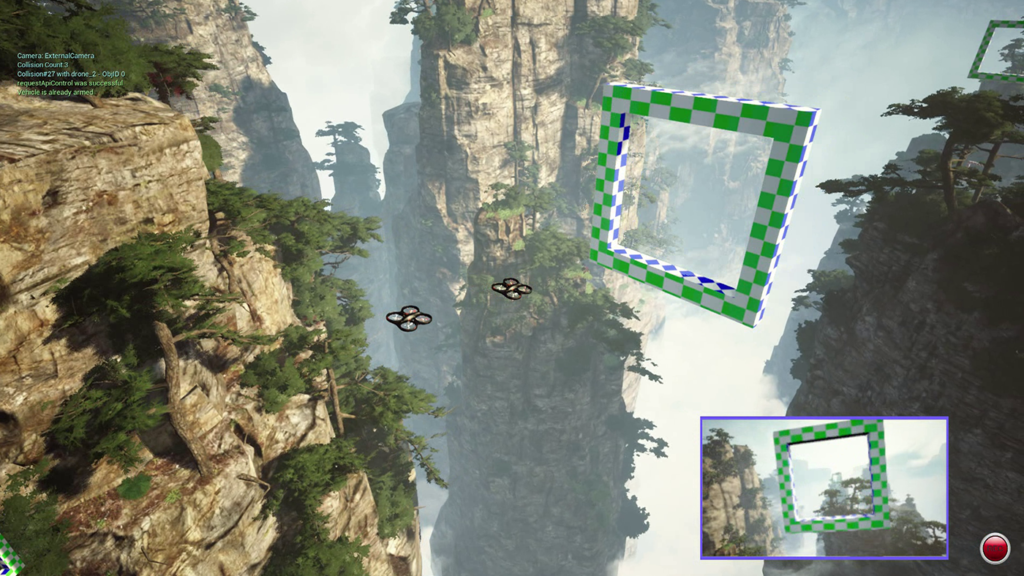
\includegraphics[width=0.75\textwidth]{imagenes/gameofdrones}
	\caption{Entorno de simulación empleado en la competición Game of Drones dentro de la conferencia NeurIPS 2019}
	\label{estado:GoD}
\end{figure}








